\documentclass[11pt,a4paper]{article}

\usepackage[T1]{fontenc}
\usepackage[utf8]{inputenc}
\usepackage[british]{babel}
\usepackage[left=0mm,right=0mm,top=0mm,bottom=0mm]{geometry}
\usepackage[stretch=25,shrink=25,tracking=true,letterspace=30]{microtype}
\usepackage{graphicx}
\usepackage{xcolor}
\usepackage{marvosym}
\usepackage{enumitem}
\setlist{parsep=0pt,topsep=0pt,partopsep=1pt,itemsep=1pt,leftmargin=6mm}
\usepackage{FiraSans}
\renewcommand{\familydefault}{\sfdefault}
\definecolor{cvblue}{HTML}{304263}

% --- Macros perso ------------------------------------------------------------
\newcommand{\dates}[1]{\hfill\mbox{\textbf{#1}}}
\newcommand{\is}{\par\vskip.5ex plus .4ex}
\newcommand{\smaller}[1]{{\small$\diamond$\ #1}}
\newcommand{\headleft}[1]{\vspace*{3ex}\textsc{\textbf{#1}}\par%
    \vspace*{-1.5ex}\hrulefill\par\vspace*{0.7ex}}
\newcommand{\headright}[1]{\vspace*{2.5ex}\textsc{\Large\color{cvblue}#1}\par%
     \vspace*{-2ex}{\color{cvblue}\hrulefill}\par}

\usepackage[colorlinks=true,urlcolor=white,linkcolor=white]{hyperref}

% -----------------------------------------------------------------------------

\begin{document}
\setlength{\topskip}{0pt}\setlength{\parindent}{0pt}\setlength{\parskip}{0pt}
\setlength{\fboxsep}{0pt}\pagestyle{empty}\raggedbottom

% ============================================================================
%                               COLONNE GAUCHE
% ============================================================================
\begin{minipage}[t]{0.33\textwidth}
\colorbox{cvblue}{\begin{minipage}[t][5mm][t]{\textwidth}\null\hfill\null\end{minipage}}
\vspace{-.2ex}
\colorbox{cvblue!90}{\color{white}
\kern0.09\textwidth
\begin{minipage}[t][293mm][t]{0.82\textwidth}\raggedright
\vspace*{2.5ex}

% ---- Identité ---------------------------------------------------------------
\Large Pape Saliou \textbf{\textsc{Fall}} \normalsize\\
\textit{Data Scientist}

\null\hfill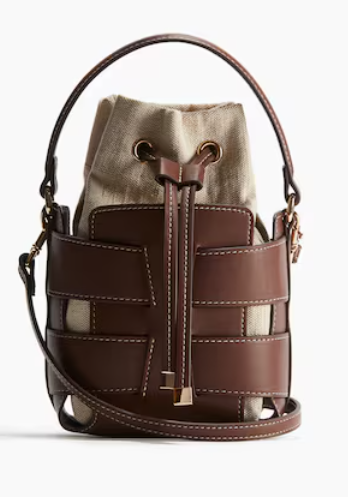
\includegraphics[width=0.65\textwidth]{38e0137e987843fea393ad1a95590721.png}\hfill\null

\vspace*{0.5ex}

% ---- Résumé -----------------------------------------------------------------
\headleft{Profile Summary}
Jeune data scientist passionné par l’extraction d’informations à forte valeur ajoutée, disposant d’un solide bagage académique en statistique, machine learning et visualisation de données. Habitué à manipuler des jeux de données complexes et à présenter des résultats clairs aux parties prenantes.

% ---- Contact ----------------------------------------------------------------
\headleft{Contact details}\small
\MVAt\ {\small papesalioufall2@gmail.com} \\[0.4ex]
\Mobilefone\ 0753481453 \\[0.5ex]
\Letter\ \href{https://www.linkedin.com/in/pape-saliou-fall-43154a211}{LinkedIn} \\[0.5ex]
\normalsize

% ---- Infos perso ------------------------------------------------------------
\headleft{Personal information}
Languages: \textbf{Français, Anglais}

% ---- Compétences ------------------------------------------------------------
\headleft{Skills}
\begin{itemize}
  \item Python
  \item R
  \item SQL
  \item Machine Learning
  \item Deep Learning
  \item NLP
  \item Power BI
  \item Data Visualization
  \item Statistiques
  \item TensorFlow
\end{itemize}

\end{minipage}\kern 0.09\textwidth
}
\end{minipage}
% ============================================================================
%                               COLONNE DROITE
% ============================================================================
\hskip2.5em
\begin{minipage}[t]{0.56\textwidth}
\setlength{\parskip}{0.8ex}
\vspace{2ex}

% ------------------------ EXPÉRIENCE ----------------------------------------
\headright{Experience}
\textsc{staigiaire en data science} at \textit{Cursanova} (Paris, France)  \dates{2022-2023} \\
\smaller{Collecte, nettoyage et préparation de jeux de données volumineux}\is
\smaller{Conception et entraînement de modèles de machine learning pour la prédiction de comportements clients}\is
\smaller{Mise en place de tableaux de bord Power BI afin de communiquer les insights aux équipes métiers}\is
\smaller{Collaboration avec les data engineers pour l’industrialisation des pipelines de données}\is

% ------------------------ ÉDUCATION ----------------------------------------
\headright{Education}
\textsc{master 1 data science}. \textit{Sorbonne Université}. \dates{2022-2023} \\

% ------------------------ CERTIFICATIONS ------------------------------------
\headright{Certifications}
\smaller{\textsc{nk}}, \textit{knp}. \dates{mai 2023} \\

% ------------------------ HOBBIES -------------------------------------------
\headright{Hobbies}
\textit{Football, Lecture, Musique}

\end{minipage}

\end{document}